\documentclass[12pt,a4paper]{article}
\usepackage[english]{babel}
\usepackage[T1]{fontenc}
\usepackage[utf8]{inputenc}
\usepackage{amsmath,amssymb}
\usepackage[hidelinks]{hyperref}
\usepackage{amsthm}
\usepackage{graphicx}
\usepackage{float}
\usepackage{mathtools}
\usepackage{geometry}
\usepackage{algorithm}
\usepackage[noend]{algpseudocode}
\usepackage{qtree}
\usepackage{subfigure}
\usepackage{listings}

\DeclareMathOperator*{\argmin}{arg\,min}
\theoremstyle{remark}
\newtheorem{ex}{Example}

\title{Wavelet\\https://fr.overleaf.com/3919739513hghwzzvxvfkt?fbclid=IwAR0UgB4-Lh6PyerPnwGu4Vc6YVpkCqPClzEqekmZ8JsoW60R_nkV3_m1V2o
\large{report}}
\author{ $\dots$ Names}

\begin{document}
\maketitle	

\section{Algorithm}

\subsection{Fast Scattering Computations}

Since in general we are dealing with big size dataset and we have to perform a lot of scattering transformation to obtain a good result in a satisfactory amount of time, we have to find a way to speed up the routine. In this section, we are going to describe a fast scattering implementation which, however, does not disperse too much of the image's energy.

The idea is to compute the windowed scattering coefficients $S[p]x$ only over frequency decreasing path,
\begin{equation*}
p= \left(  2^{-j_1} r_1, \dots , 2^{-j_m} r_m \right) \quad \text{such that } 0 < j_k \leq j_{k+1} \leq J \, ,
\end{equation*} 
on which is concentrated almost all of the scattering energy.

In a general setting, if the wavelet transform is computed over $K$ rotation angles and over path of maximum length $\overline{m}$, then the total number of frequency-decreasing paths of length $m$, i.e. $\mathcal{P}_{\downarrow }^{m}$, is  $K^{m} {J \choose m}$. 

\begin{ex}
	For a better understanding, let us consider a simple invariant scattering convolution network with $m=3$ layers, no rotations ($K=1$) and maximal space scale parameter $J=3$. With these settings, the network will output $8$ scattering coefficient which are given by:
	\begin{itemize}
	\item ${J \choose 0} = 1$ path of length $0$: $\emptyset$;
	\item ${J \choose 1} = 3$ paths of length $1$: $(2^{-1}),(2^{-2}),(2^{-3})$;
	\item ${J \choose 2} = 3$ paths of length $2$: $(2^{-1},2^{-2}),(2^{-1},2^{-3}),(2^{-2},2^{-3})$;
	\item ${J \choose 3} = 1$ path of length $3$: $(2^{-1},2^{-2},2^{-3})$;
	\end{itemize}
	and they will be computed like this:
	\begin{center}
	\Tree[.$S[\emptyset]x=x\star\Phi_{2^3}$ [.$S[(2^{-1})]x$ [.$S[(2^{-1},2^{-2})]x$ [.$S[(2^{-1},2^{-2},2^{-3})]x$ ] ]
	[.$S[(2^{-1},2^{-3})]x$ ]]
	[.$S[(2^{-2})]x$ [.$S[(2^{-2},2^{-3})]x$ ]][.$S[(2^{-3})]x$ ]]
	\end{center}
\end{ex}

Now, let $N$ be the number of pixels of a given image $x$, since $\Phi_{2^J}$ is a low-pass filter scaled by $2^J$, we obtain that $S[p]x(u) = U[p]x \star \Phi_{2^J}(u)$ is uniformly sampled at intervals $2^J$. Moreover, we can even decide to sample at higher frequency using intervals of the form $\alpha2^J$ with $\alpha = \frac{1}{2}$ to exploit the oversampling, which is a technique that lowers the error and improve resolutions. So, each scattering coefficient
$S[p]x$ is an image itself with an amount of $\alpha^{-2} 2^{-2J} N$ coefficients.
To have a better idea on how the choices of these parameters influent the scattering coefficients, take a look at figure (\ref{JA}), where a simple example is shown.

\begin{figure}[H] \label{JA}
	\centering
	\subfigure{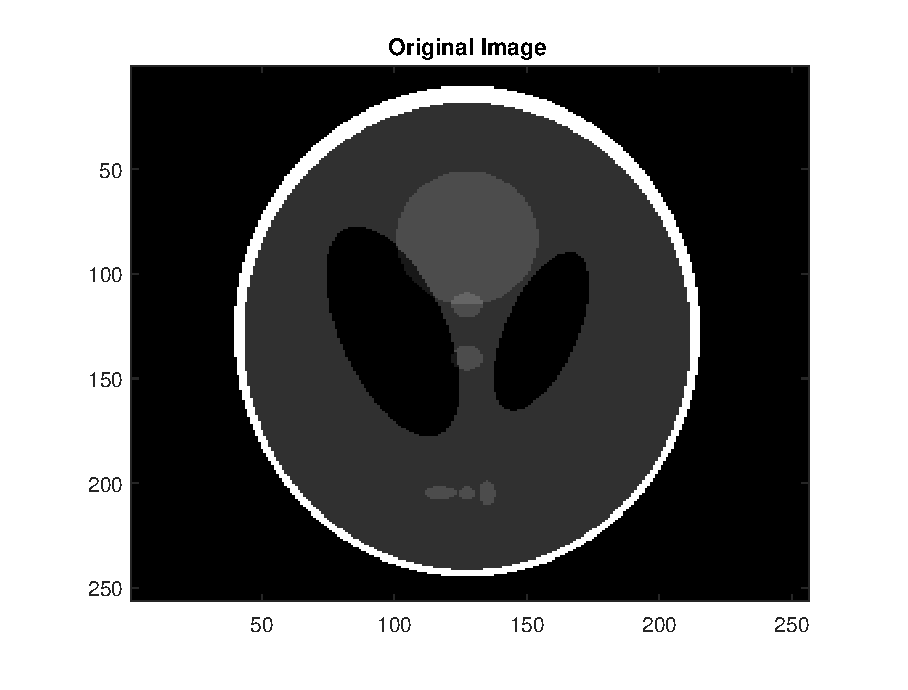
\includegraphics[width=0.5\linewidth, height=0.18\textheight]{img/OI}} \\
	\subfigure[$J=1$, we obtain $16384$ coefficients.]{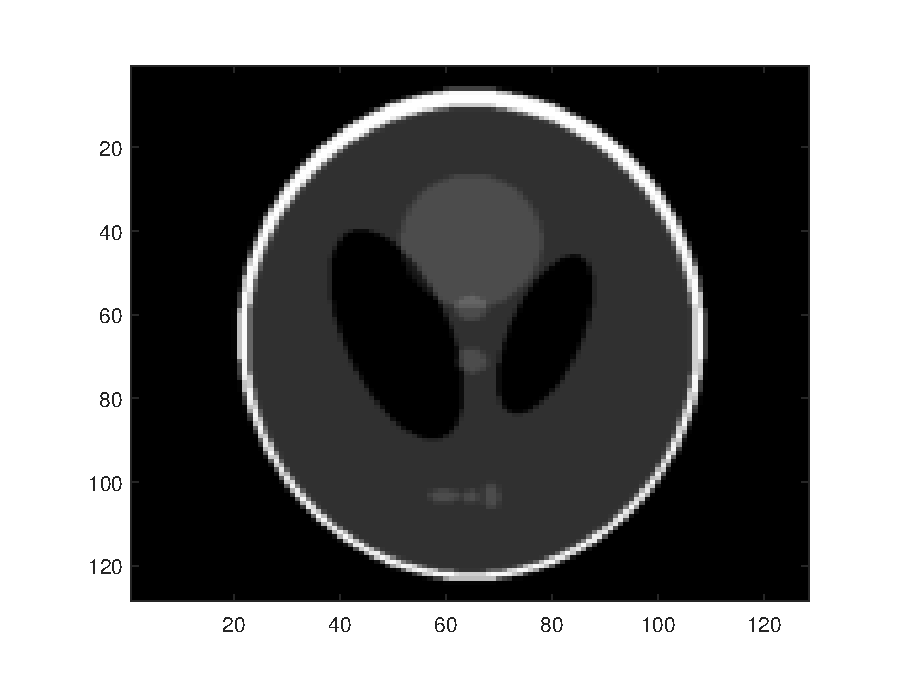
\includegraphics[width=0.45\linewidth, height=0.17\textheight]{img/J1_O0A1}}
	\subfigure[$J=1$, we obtain $65536$ coefficients.]{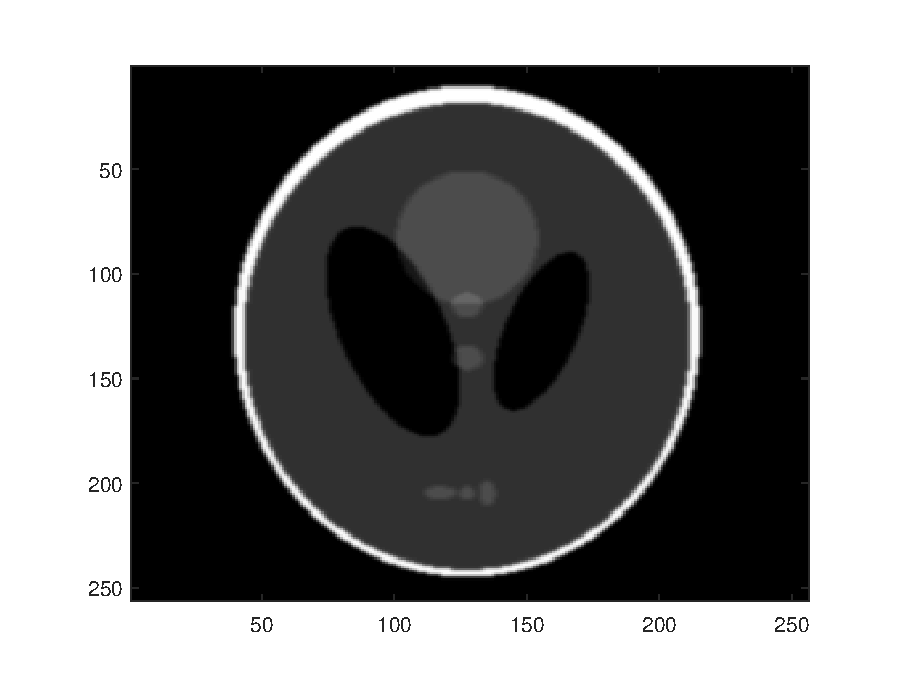
\includegraphics[width=0.45\linewidth, height=0.17\textheight]{img/J1_O1A12}}\\
	\subfigure[$J=4$, we obtain $256$ coefficients.]{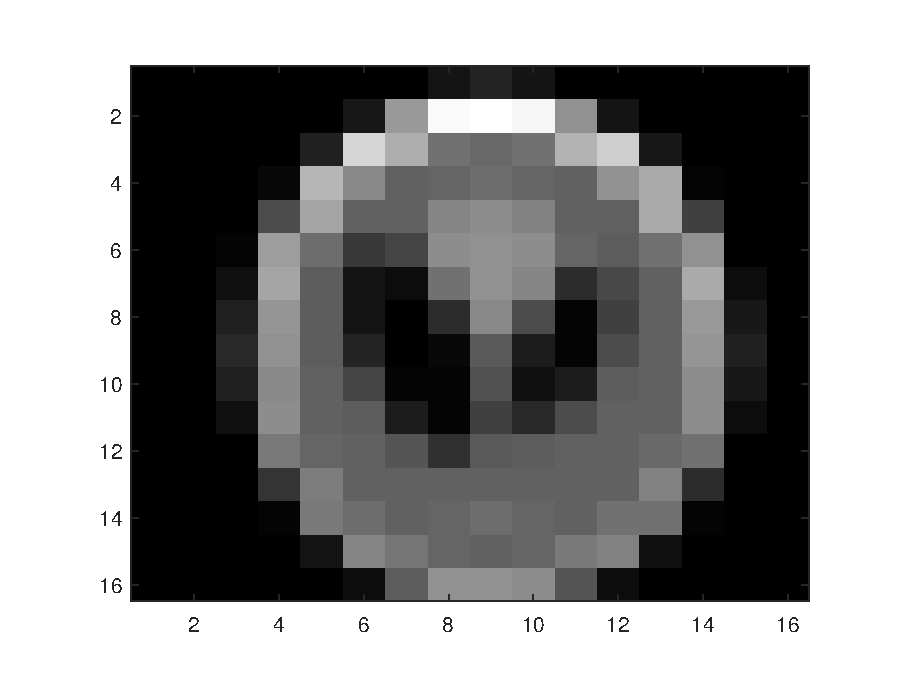
\includegraphics[width=0.45\linewidth, height=0.17\textheight]{img/J4_O0A1}}
	\subfigure[$J=4$, we obtain $1024$ coefficients.]{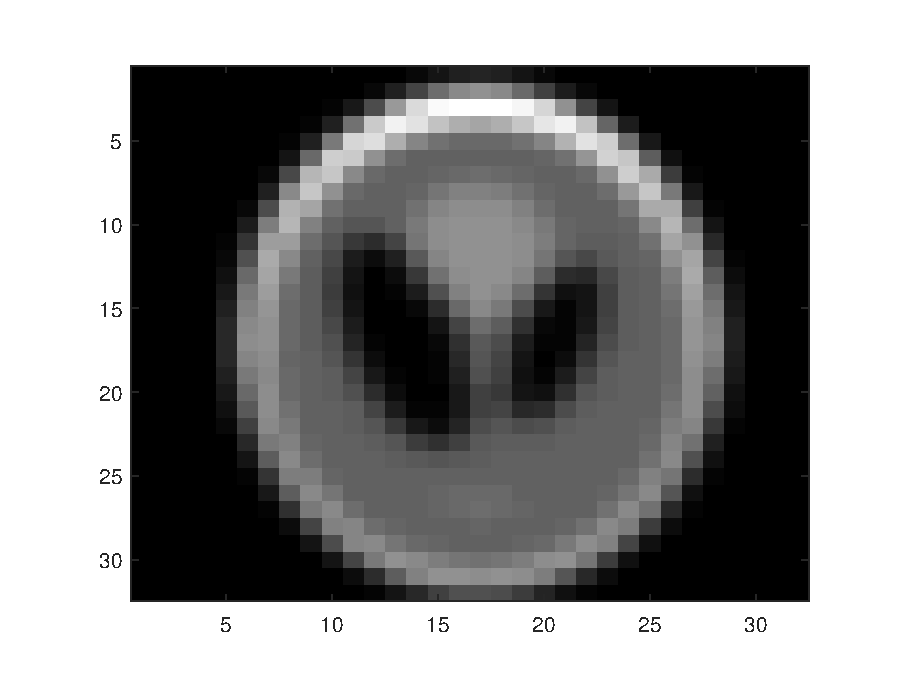
\includegraphics[width=0.45\linewidth, height=0.17\textheight]{img/J4_O1A12}}\\
	\subfigure[$J=8$, we obtain $1$ coefficient.]{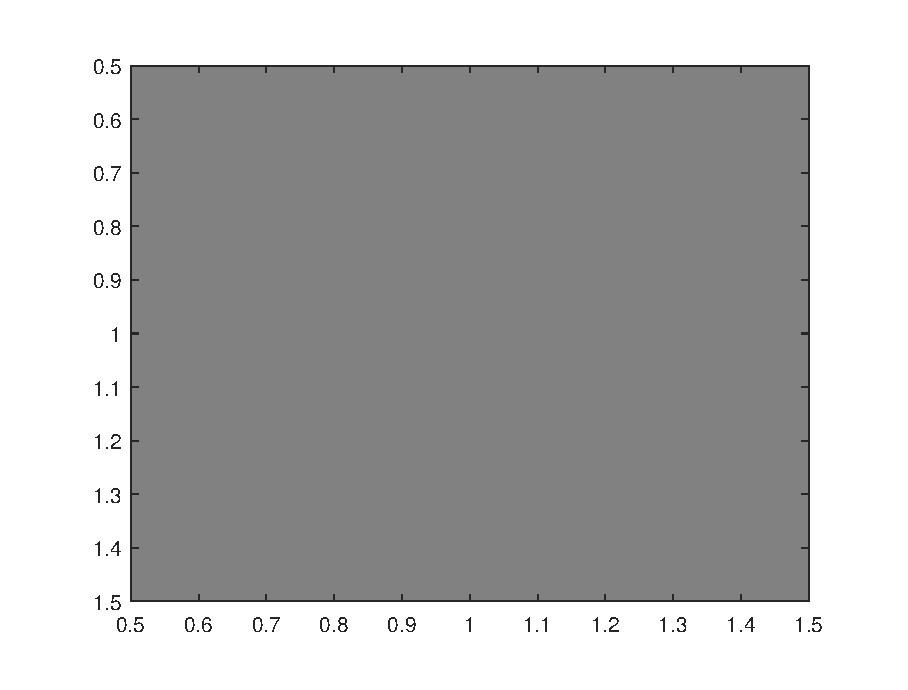
\includegraphics[width=0.45\linewidth, height=0.17\textheight]{img/J8_O0A1}}
	\subfigure[$J=8$, we obtain $4$ coefficients.]{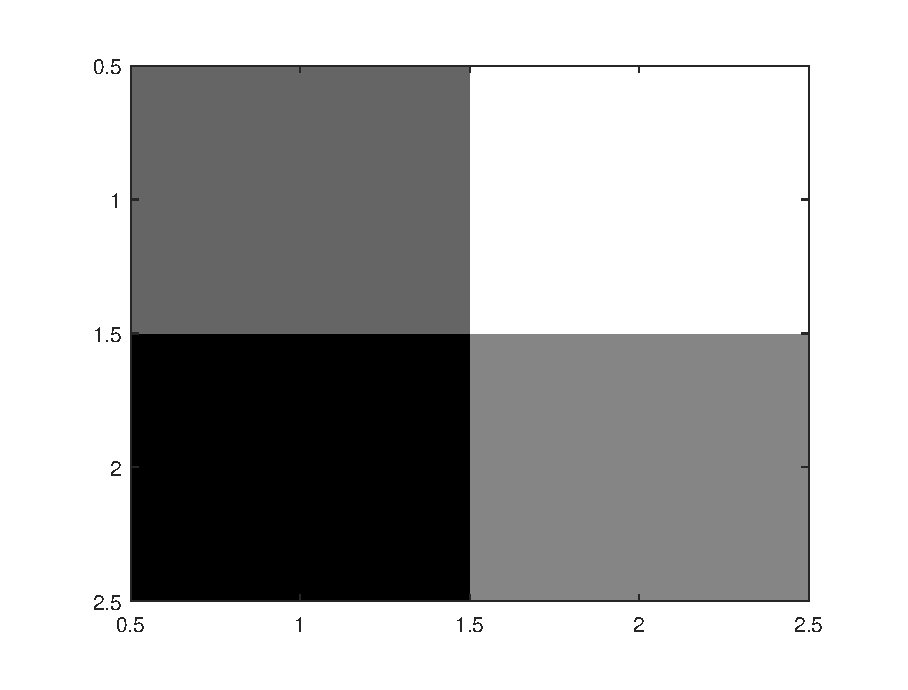
\includegraphics[width=0.45\linewidth, height=0.17\textheight]{img/J8_O1A12}}
	\caption{In this figure are shown the original image $x$ (at the top) with $N = 2^8 \times 2^8 = 65536$ pixels and various windowed scattering coefficients of order $0$ for different choices of the maximal space scale $2^J$. In the left column, we decided not to perform oversampling (i.e. $\alpha =1$), while we did it in the right one ($\alpha = \frac{1}{2}$).}
\end{figure}


Finally, the total number of coefficients in a scattering network $P$ is given by the number of coefficient per layer and the number of layers, more precisely
\begin{equation*}
P= \alpha^{-2} 2^{-2J} N \sum_{m=0}^{\overline{m}} K^{m} {{J}\choose{m}} \,.
\end{equation*}

Algorithm (\ref{FST}), reported below, describes the computation of scattering coefficients on sets $\mathcal{P}_{\downarrow}^{m}$ of frequency decreasing paths of length $\overline{m}$. The initial set correspond to the original image, $U[\emptyset]x=x$, and we can choose to sub-sample convolutions at interval $\alpha2^j$, with $\alpha=1$ or $\alpha=\frac{1}{2}$, to avoid aliasing.

\begin{algorithm}
	\caption{Fast Scattering Transform}\label{FST}
	\begin{algorithmic}[1]
		\Procedure{}{}
		\For {$m=1$ to $\overline{m}$}
		\ForAll {$p \in \mathcal{P}_{\downarrow}^{m-1}$}
		\State Output $S[p]x (\alpha 2^J N) = U[p]x \star \Phi_{2^J}(\alpha 2^J N)$
		\EndFor
		\ForAll {$p+\lambda_m \in \mathcal{P}_{\downarrow}^{m}$ with $\lambda_m = 2^{-j_m}r_m$}
		\State Compute  $U[p+\lambda_m]x (\alpha 2^{j_m} N) = | U[p]x \star \psi_{\lambda_m}(\alpha 2^{j_m} N) |$ 
		\EndFor
		\EndFor
		
		\ForAll {$p \in \mathcal{P}_{\downarrow}^{\overline{m}}$}
		\State Output $S[p]x (\alpha 2^J N) = U[p]x \star \Phi_{2^J}(\alpha 2^J N)$
		\EndFor
		\EndProcedure
	\end{algorithmic}
\end{algorithm}

On could verify by induction over the number of layer $m$ (and using the estimates from before), that the total amount of samples of the propagated signals $U[p]x$ in the $m^{\text{th}}$ layer, with $p \in \mathcal{P}_{\downarrow}^{m}$,  is equal to $\alpha^{-2} \left(\frac{K}{3}\right)^m N$. Similarly, one can calculate the amount of scattering signals' coefficients $S[p]x$, which are much fewer since the are sub-sampled by $2^J$.

Thus, the number of operations realized to compute each layer $m$ is of the order of $O( \left( \frac{K}{3}\right)^m N \log N)$, and they are needed to compute the internal propagated coefficients with FFTs. For $K>3$, the overall computation complexity is thus $O( \left( \frac{K}{3}\right)^{\overline{m}} N \log N)$.

\subsection{Understanding of the algorithm}
To gain a better knowledge of the subject and in order to compare this new method with other image classification ones, like CNNs, we were asked to understand the \textit{ScatNet Software} to be able to exploit it in our classification simulations. This software is already implemented in MATLAB by the \textit{Data Team} of the Ecole Normale Superieure of Paris, whose scientific leader is Stéphane Mallat.

It is a scattering transform builds invariant, stable and informative signal representations for classification. It is computed by scattering the signal information along multiple paths, with a cascade of wavelet modulus operators. It is implemented in a deep convolutional network and it is stable to deformations, which makes it particularly effective for image discrimination. Now, let us see more in specific how it works.

First of all, we have to decide the characteristic of our Network, and we can do it by setting the options with the following commands:
\begin{description}
	\item[filt\_opt.J] let us define the parameter $J$, which determine the maximal scale of the spatial variability and the size of the spatial windows $\Phi_{2^J}$;
	\item[filt\_opt.L] let us define the parameter $K$, which determines the group of positive rotations $G_{+}= \{ r = \frac{k\pi}{K} | 0\leq k < K \}$, since images are real-valued signal;
	\item[scat\_opt.M] let us define the parameter $\overline{m}$, that is the maximal order of the network and that fix the limit length of each path;
	\item[scat\_opt.oversampling] let us decide if we want to perform oversampling by setting the parameter equals to $1$ (yes) or $0$ (no).
\end{description}

At this point, we can generate the wavelets' operator exploiting the function :
\begin{lstlisting}
[Wop,filters] = wavelet_factory_2d(size(x),filt_opt,scat_opt); 
\end{lstlisting}
whose inputs are the dimension of the image and the parameters we just defined. On the other hand, the output are
\begin{description}
	\item[Wop] a cell array of function handles, i.e. a cell array containing all the linear operators, grouped for each layer $m$, which are involved in the scattering network,	
	\item[filters]  a structure array (called struct) containing the fields
	\begin{description}
		\item[phi] a struct containing all the informations on the lower-pass filter $\Phi$,
		\item[psi] a struct containing all the informations on the dilated and oriented wavelets $\Psi$,
		\item[meta]a struct containing the global information about the filter bank.
	\end{description}
\end{description}

Lastly, we can exploit the command
\begin{lstlisting}
[S,V] = scat(x, Wop);
\end{lstlisting}
which is applied layer by layer and for each of them compute
\begin{description}
	\item[S]  the scattering coefficients at the actual layer,
	\item[V] the translation invariant coefficient of the next one.
\end{description} 

\begin{figure}[ht]
	\centering
	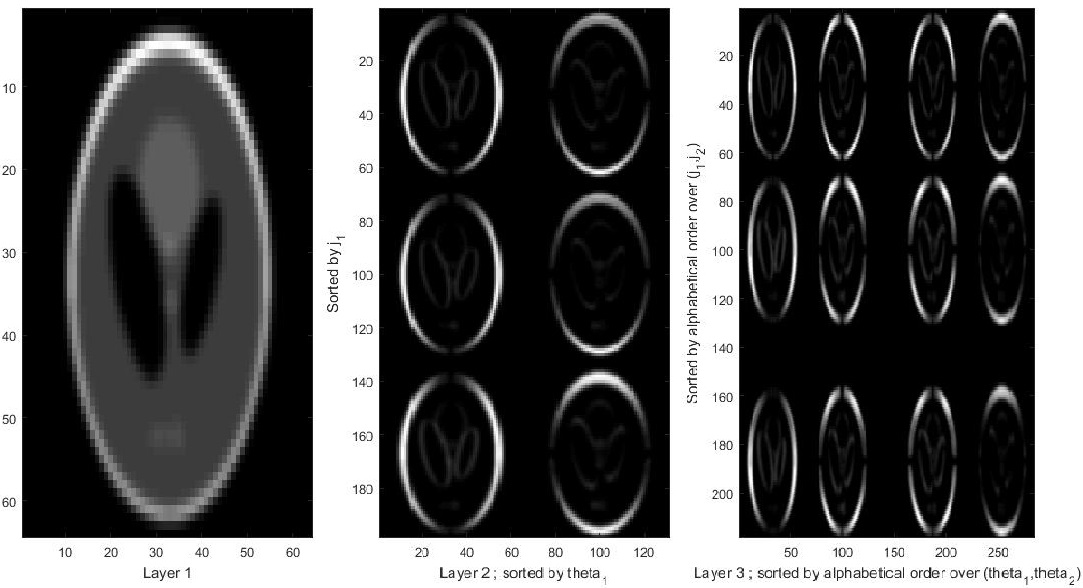
\includegraphics[width=1\linewidth, height=0.35\textheight]{img/J3L2M2O1_2}
	\caption{In the Figure are shown the scattering coefficients of the same image depicted in Figure (\ref{JA}) with respect to a network having $\overline{m} = 2$ layers, maximal space scale $J=3$ and $K=2$ positive rotations.
	In the picture on the left are shown the coefficient of the  layer $m=0$, that is the convolution between the original image $x$ and the lower-pass filter $\Phi_{2^3}$.
	In the second picture are displayed the coefficient of the first layer ordered in increasing order with respect to $j_1$ (top to bottom) and $r_1$ (left to right). 
	In the third one appear the coefficients of the last layer $m=2$ sorted in increasing order over the couple $(j_1, j_2)$ (top to bottom) and $(r_1, r_1)$ (left to right). We can notice that only the coefficients over frequency decreasing paths are computed and we have $ {\sum_{m=0}^{2} 2^m {{3}\choose{m}}} = 19$ of them.}
	\label{fig:j3l2m2o1}
\end{figure}

\section{Convolutional Neural Networks} % How detailed should the explanation of CNNs be? 

Convolutional Neural networks (CNN) are commonly considered as the state of the art tool for image classification. In this section we will briefly describe the theoretical concepts of a CNN. Then we will describe our implemented architecture and the performance of our trained network on the MNIST data set.
\subsection{Theory} % needs some references
Just like with traditional NN CNN:s consist of several layers which of weight matrices and some additional operations, activation, pooling etc. In CNNs the learned weights represents  so called filters or kernels that are convoluted with the input to each hidden layer to transform the input to some feature space where the class separation is large. In addition to the convolutions at each layer the input is passed through some non-linear activation function, usually a Rectified Linear Unit (ReLU), to enable the network to handle non-linearly separable problems. 

The main difference between traditional neural networks (NN) and CNN:s are the following points

\begin{itemize}
\item Local connectivity 
\item Weight sharing
\item Translation invariance
\item Arbitrary input size
\end{itemize}

Local connectivity means that the nodes in the network are only connected to neighbouring nodes instead of all nodes in the previous layers. This  reduces the required amount of parameters compared to a traditional NN. Since image data is very high dimensional the local connectivty is an important feature. The shared weights also decreases the amount of parameters since the nodes shares the same weights, or filters, instead of having unique weights for each node. The translation invariance means that the CNN makes the same prediction no matter where in the image an object is located. The feature of arbitrary input size makes it easier to adapt the network to different kinds of data, eg. different image sizes. 

\subsection{Our implementation}
As a reference network to compare with our wavelet scattering network we used a two layer CNN implemented with the Python library Keras. This architecture is not fully optimized since we only wanted it as a reference point for the wavelet network. More complex and finetuned architectures could have been used to really optimize the prediction performance. This architecture has around 500 000 trainable parameters which can be compared to XX which is the number of parameters in the svd classifier used in the wavelet scattering networks. 

\begin{lstlisting}[language=Python, caption={Calculation of moments}]
# Network structure
    model = Sequential()
    model.add(Conv2D(16, kernel_size=(5, 5), strides=(1, 1), padding='same',
                     activation='relu', input_shape=input_shape))
    model.add(BatchNormalization(axis=1))
    model.add(MaxPooling2D(pool_size=(2, 2)))
    model.add(Conv2D(32, kernel_size=(3, 3), strides=(1, 1), padding='same',
                     activation='relu'))
    model.add(BatchNormalization(axis=1))
    model.add(MaxPooling2D(pool_size=(2, 2)))
    model.add(Flatten())
    model.add(Dense(300, activation='relu'))
    model.add(Dense(num_classes, activation='softmax'))

    model.compile(loss=keras.losses.categorical_crossentropy,
                  optimizer=optimizers.Adam(lr=0.001, beta_1=0.9, beta_2=0.999, epsilon=None, 
                  decay=0.001,amsgrad=False),metrics=['accuracy'])

\end{lstlisting}

\subsection{Results} % We can make some experiments with less data to see if the wavelet scattering can outperform the CNN for low sample size. Could be a motivation for scattering networks. Still get 97,9 % acc when using 10% of the training set. 91% when using 1% of the training set. 

After one epoch of training on the entire MNIST training set the model achieves 98.6\% accuracy on the test set


\end{document}